\section{Критерий решёточной раскраски и протокол точной проверки}
\label{sec:method}

\subsection{Решётки, ячейки Вороного, раскраска классами смежности}

\emph{Решётка} $\Lambda\subset\R^n$ --- множество всех целочисленных линейных
комбинаций $n$ линейно независимых векторов $b_1,\dots,b_n$ (базиса).
\emph{Подрешётка} $\Gamma\subseteq\Lambda$ --- решётка, все узлы которой лежат
в $\Lambda$; её \emph{индекс} $k=[\Lambda:\Gamma]$ равен числу классов
смежности $\Lambda/\Gamma$ и вычисляется как модуль определителя
целочисленной матрицы перехода. \emph{Ячейкой Вороного} узла $a\in\Lambda$
называется множество точек, для которых $a$ --- ближайший узел:
\[
V_\Lambda(a)=\{x\in\R^n:\ \|x-a\|\le\|x-b\|\ \ \forall b\in\Lambda\}.
\]
Это выпуклый многогранник; все ячейки одинаковы с точностью до сдвига и
вместе замощают $\R^n$. Обозначим $V_0=V_\Lambda(0)$.

\begin{figure}[t]
\centering
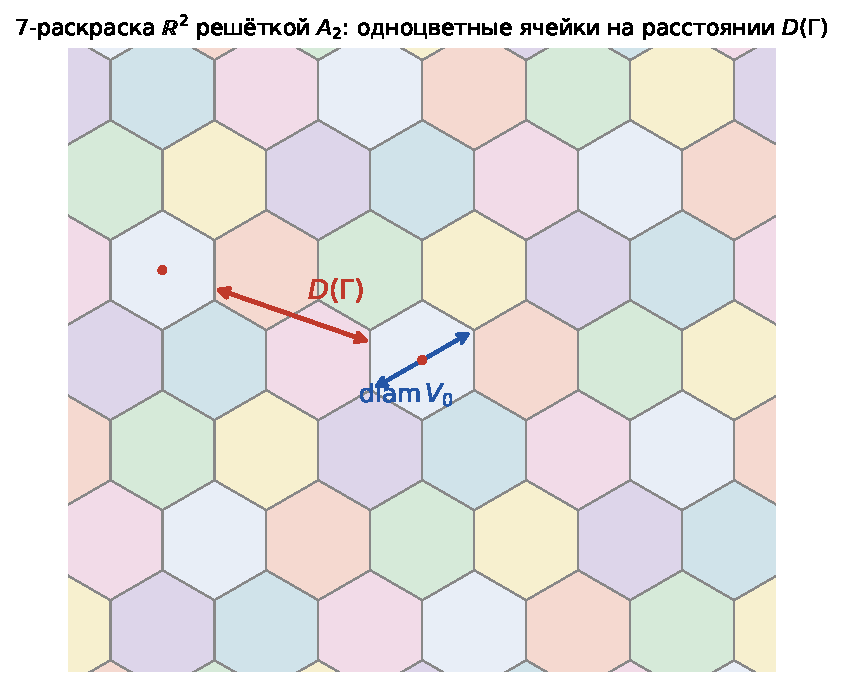
\includegraphics[width=0.62\textwidth]{fig_method.pdf}
\caption{Идея метода на примере $7$-раскраски плоскости шестиугольной решёткой
$A_2$ (конструкция Исбелла, $\chi(\R^2)\le7$). Каждая ячейка Вороного
окрашена цветом своего класса смежности по подрешётке индекса~$7$. Две
\emph{одноцветные} ячейки (красные точки) разделены расстоянием $D(\Gamma)$,
строго большим диаметра ячейки $\diam V_0$; раскраска запрещает все
расстояния из промежутка $\bigl(\diam V_0,\,D(\Gamma)\bigr)$.}
\label{fig:method}
\end{figure}

Зафиксируем подрешётку $\Gamma\subseteq\Lambda$ индекса $k$ и окрасим каждую
ячейку $V_\Lambda(v)$ цветом класса смежности $v+\Gamma$; получается
$k$-цветная периодическая раскраска $\R^n$ (рис.~\ref{fig:method}). Две точки
одного цвета лежат либо в одной ячейке, либо в ячейках $V_\Lambda(a)$,
$V_\Lambda(b)$ с $v=a-b\in\Gamma\setminus\{0\}$. В первом случае расстояние
не превосходит $\diam V_0$, во втором --- не меньше расстояния между
ячейками. Обозначим
\[
D(v)=\dist\bigl(V_0,\,v+V_0\bigr),\qquad
D(\Gamma)=\min_{v\in\Gamma\setminus\{0\}}D(v),\qquad
d(\Lambda,\Gamma)=\frac{D(\Gamma)}{\diam V_0}.
\]
Множество реализуемых одноцветных расстояний лежит в
$[0,\diam V_0]\cup[D(\Gamma),\infty)$, а открытый промежуток
$(\diam V_0,D(\Gamma))$ \emph{свободен}.

\begin{proposition}\label{prop:crit}
Если $d(\Lambda,\Gamma)>1$, то $\chi\bigl(\R^n,[1,\ell]\bigr)\le[\Lambda:\Gamma]$
при всех $\ell<d(\Lambda,\Gamma)$; в частности $\chi(\R^n)\le[\Lambda:\Gamma]$.
\end{proposition}
\begin{proof}
Возьмём масштаб $s>0$ с $s\,\diam V_0<1$ и $s\,D(\Gamma)>\ell$ --- это возможно
тогда и только тогда, когда $\ell<D(\Gamma)/\diam V_0=d$. Для решётки $s\Lambda$
свободный промежуток $\bigl(s\diam V_0,\,sD(\Gamma)\bigr)$ содержит весь отрезок
$[1,\ell]$, значит, раскраска правильна для $[1,\ell]$. Случай $\ell=1$ (с учётом
\eqref{eq:mono}) даёт $\chi(\R^n)\le k$.
\end{proof}

Величину $d$ называем \emph{нормированной шириной} запрещённого интервала.
Наименьшее число цветов среди раскрасок описанного вида принято обозначать
$\chi_s\bigl(\R^n,[1,\ell]\bigr)$; все известные верхние оценки в малых
размерностях, включая доказанные ниже, --- это оценки на $\chi_s$.

\begin{remark}[о границах ячеек]\label{rem:halfopen}
Ячейки Вороного замкнуты и пересекаются по границам, поэтому <<окрасим каждую
ячейку>> само по себе не задаёт функцию на $\R^n$. Как обычно, фиксируем
полуоткрытую фундаментальную область: из каждой пары соседних ячеек общая
грань приписывается одной из них. Оценки от этого выбора не зависят, так как
диаметр полуоткрытой ячейки не превосходит $\diam V_0$, а расстояние между
различными одноцветными ячейками не меньше $D(v)$.
\end{remark}

\subsection{Лемма о середине и окно полноты}

Ячейка $V_0$ --- выпуклый центрально-симметричный многогранник, и все её
фасеты центрально-симметричны (Вороной~\cite{Voronoi}); в частности
$\diam V_0=2R$, где $R=\max_{x\in V_0}\|x\|$ --- радиус покрытия. Центральная
симметрия сводит расстояние между двумя многогранниками к расстоянию от точки
до одного из них.

\begin{lemma}[о середине; {\cite[лемма~2]{Ivanov2011}}]\label{lem:mid}
Минимальное расстояние между $V_0$ и $v+V_0$ реализуется на паре точек,
симметричных относительно середины $v/2$ отрезка центров, поэтому
\begin{equation}\label{eq:mid}
D(v)=2\,\dist\bigl(v/2,\,V_0\bigr).
\end{equation}
\end{lemma}
\begin{proof}[Идея]
Пусть минимум достигается на $x\in V_0$, $y\in v+V_0$. Отражение относительно
$v/2$ переводит $V_0$ в $v+V_0$ и наоборот; образы $x',y'$ дают ту же длину.
Середины отрезков $[x,y']$ и $[y,x']$ по выпуклости лежат в соответствующих
ячейках, симметричны относительно $v/2$ и реализуют то же минимальное
расстояние; расстояние от каждой из них до $v/2$ равно $\dist(v/2,V_0)$.
\end{proof}

Минимум $D(\Gamma)$ берётся по бесконечной подрешётке, но перебирать нужно
конечное множество. Так как $V_0$ содержится в шаре радиуса $R=\frac12\diam V_0$,
справедливо $D(v)\ge\|v\|-\diam V_0$. Поэтому нарушить неравенство
$D(v)\ge\ell\diam V_0$ может лишь вектор с
\begin{equation}\label{eq:window}
\|v\|\ <\ (1+\ell)\diam V_0=2(1+\ell)R ,
\end{equation}
и это \emph{доказуемо полная} граница перебора: она не зависит от базиса
подрешётки. (Более узкое окно $\|v\|<4R$ отвечало бы лишь цели $d>1$ и для
интервального утверждения недостаточно.)

\subsection{Протокол точного сертификата}\label{ssec:protocol}

Три теоремы \S\ref{sec:constr} доказываются по одной схеме: численный
оптимум, найденный поиском (\cite[\S3]{Full}), округляется до рациональной
решётки, и дальше проверяется \emph{именно эта} решётка. Происхождение
кандидата на доказательство не влияет; влияет только приведённый ниже
конечный список проверок, каждая из которых выполняется в точной арифметике
дробей.

\begin{proposition}[протокол сертификата]\label{prop:protocol}
Пусть $Q\in\mathrm{Mat}_n(\Q)$ --- симметричная матрица с положительными
главными угловыми минорами, $\Lambda=\Z^n$ со скалярным произведением
$\langle x,y\rangle=x^{\mathsf T}Qy$, и $\Gamma=C\Z^n$ для целочисленной
$C$. Пусть конечная проверка установила:
\begin{enumerate}[leftmargin=2.2em,itemsep=1pt,label=\textup{(\roman*)}]
\item \emph{индекс}: $|\det C|=k$;
\item \emph{фасеты}: для каждого из $2^n-1$ ненулевых классов $\Lambda/2\Lambda$
найдены кратчайшие представители; классы с единственной парой $\pm v$
кратчайших дают список релевантных векторов $v$, и $V_0$ задаётся
неравенствами $\langle x,v\rangle\le\frac12\langle v,v\rangle$ по этому списку;
\item \emph{вершины}: перечислены все вершины $V_0$, причём полнота
доказана либо перебором всех $n$-подмножеств фасет, либо точным замыканием
по одномерному скелету; $R^2=\max\langle x,x\rangle$ по вершинам и
$\diam^2V_0=4R^2$;
\item \emph{окно}: перечислены все $v\in\Gamma\setminus\{0\}$ с
$\langle v,v\rangle<W$, где $W\ge\bigl(2(1+\ell_0)R\bigr)^2$ --- рациональная
граница;
\item \emph{разделение}: для каждого $v$ из окна предъявлены точка
$x^*\in V_0$ (допустимость проверена по всем фасетам) и множители
$\mu\ge0$ активных фасет с $v/2-x^*=\sum\mu_jv_j$, откуда
$D(v)^2=4\langle v/2-x^*,v/2-x^*\rangle$ точно;
\item \emph{запас}: $D_{\min}^2-\ell_0^2\,\diam^2V_0>0$ как рациональное число,
где $D_{\min}$ --- минимум по окну.
\end{enumerate}
Тогда $d(\Lambda,\Gamma)>\ell_0$ и $\chi\bigl(\R^n,[1,\ell]\bigr)\le k$ при
всех $\ell\le\ell_0$.
\end{proposition}

\begin{proof}
(ii)~--- теорема Вороного о релевантных векторах: $v$ задаёт фасету тогда и
только тогда, когда $\pm v$ --- единственная пара кратчайших представителей
класса $v+2\Lambda$; граница перебора внутри класса полна, поскольку у каждого
класса есть представитель с координатами из $\{0,1\}$, а кратчайший не длиннее
его. (iii)~--- максимум выпуклой функции $\langle x,x\rangle$ по многограннику
достигается в вершине; $\diam V_0=2R$ по центральной симметрии.
(iv)~--- окно~\eqref{eq:window}: вектор вне окна удовлетворяет
$D(v)\ge\|v\|-\diam V_0\ge\ell_0\diam V_0$ автоматически. (v)~--- условия
Каруша--Куна--Таккера достаточны для выпуклой задачи проекции на многогранник,
а по лемме~\ref{lem:mid} $D(v)=2\dist(v/2,V_0)$. (vi)~вместе с (iv), (v) даёт
$D(\Gamma)>\ell_0\diam V_0$, и остаётся предложение~\ref{prop:crit}.
\end{proof}

Дополнительный контроль, применяемый во всех сертификатах: центральная
симметрия множества вершин, соотношение Эйлера для $f$-вектора и равенство
$\vol V_0=\det\Lambda$. Плавающая точка используется лишь как
\emph{оракул-подсказчик} (перечислитель предлагает вершину, решатель --- активный
набор проекции); каждая принятая величина пересчитывается над $\Q$, поэтому
ошибка оракула может лишь остановить проверку, но не сделать её неверной.
